\chapter{Statistical testing\label{ch:statistical}}

\graphicspath{{figs/statistical/}}

The $p$-value approach to statistical hypothesis testing consists of the following five steps \shortcite{ewens2004statistical}. 
\\ \\{\bf Step 1} is to state the \emph{null hypothesis} ($H_0$) and the \emph{alternative hypothesis} ($H_1$). The aim is to either reject or accept $H_0$. Accepting $H_0$ does not mean that it is necessarily true, only that there was insufficient evidence against it.
\\ \\{\bf Step 2} is to determine the \emph{level of significance} $\alpha\label{eq:alpha}$. This is the probability of making a \emph{type I error}, i.e., rejecting $H_0$ when it is true. We obviously want this probability to be small, but a too small $\alpha$ will increase the probability $\beta\label{eq:beta}$ of making a \emph{type II error}, i.e., accepting $H_0$ when it is false. The choice of $\alpha$ will therefore depend on the situation and what type of error is most important for us to avoid. 
\\ \\{\bf Step 3} is to decide on a \emph{test statistic} $T$. Which test statistic is used depends on the situation. 
\\ \\{\bf Step 4} is to compute the value $t_\text{obs}$ of this test statistic from the observations.
\\ \\{\bf Step 5} is to compute the $p$-value, i.e., the probability that the test statistic $T$ would have a value at least as extreme as the observed value $t_\text{obs}$ under $H_0$. If the alternative hypothesis corresponds to large values of $T$, the $p$-value is calculated as $\Prob{T \ge t_\text{obs}}$. Thus, roughly speaking, a small $p$-value indicates that $H_0$ is unlikely. The $p$-value is compared with the chosen level of significance $\alpha$ (typically 0.05 or 0.01). If the $p$-value it is smaller, $H_0$ is rejected, otherwise, $H_0$ is accepted.
\\ \\
When the test statistic is continuous, the $p$-value is a continuous, random variable with a uniform distribution $\mathcal{U}(0, 1)\label{eq:uniform}$ under $H_0$ \shortcite{ewens2004statistical}, meaning it will satisfy the equation
\begin{equation}
\ProbCond{\text{$p$-value} \le x}{H_0 \;\text{true}} = x
\end{equation}
for $x \in [0,1]$. When the test statistic is \emph{discrete}, the $p$-value is also discrete, but it is \emph{not} discrete \emph{uniform} under $H_0$. The reason is that a $p$-value that satisfies the equation above might not exist. Instead, the $p$-value will satisfy 
\begin{equation}
\ProbCond{\text{$p$-value} \le x}{H_0 \;\text{true}} \le x.
\end{equation}
The deviation from the uniform distribution is large when data is sparse, but for larger data sets, the deviation is often negligible. 

In certain situations, a \emph{two-level test procedure} is advantageous. First, the expected distribution is compared with the empirical distribution observed, using some goodness-of-fit (GOF) tests. In accordance with classical hypothesis testing, a failure to pass such a test at some level of significance $\alpha$ would result in the rejection of the null hypothesis $H_0$ that the empirical frequencies follow the expected distribution, with a probability $\alpha$ of making a type I error. Successfully passing a test would typically cause $H_0$ to be accepted, with a probability $\beta$ of making a type II error. $\beta$ is often quite large. We might therefore want to run the test several times before we feel confident that $H_0$ can be accepted. When doing experiments on a computer, the cost of re-running the test is usually small. We can, therefore, run the experiment a large number of times, and check whether the test fails the expected fraction $\alpha$ of the tests. But this way we would lose a lot of information, and it is arguably not the best approach in this situation. In the case where the $p$-value is (sufficiently) uniform under $H_0$, we can instead test the observed $p$-values generated against the expected $\mathcal{U}(0, 1)$. This approach, sometimes referred to as a \emph{two-level test procedure}, is similar to the one used by \citeN{lecuyer2007testu01} to test PRNGs. The test of the $p$-values will of course have its own $p$-value, which in turn could be compared to the expected uniform distribution using some GOF test, and so on, repeating endlessly. Nevertheless, it should suffice to do one test against uniformity, and compare the resulting $p$-value to some predefined level of significance $\alpha$. The main advantage of this two-level approach is that if a connection algorithm passes the test, our confidence in it will be much greater than if only a single test was performed. 

The GOF test used in the first step of the procedure will vary depending on the data. The tests we will use are introduced below. For the second step (the test of GOF of the $p$-values to $\mathcal{U}(0, 1)$) the Kolmogorov-Smirnov test is used.



\section{Pearson's chi-squared test\label{sec:chi}}

The following section is based on \emph{A Guide to Chi-Squared Testing} \shortcite{greenwood1996guide}.
Pearson's chi-squared test, sometimes ambiguously referred to as ``the chi-squared test'', is a test of the null hypothesis that there is a good fit between some theoretical distribution and the observed data.

Consider an experiment, or \emph{trial}, resulting in one outcome, $A_i\label{eq:Ai}$, of $r\label{eq:r}$ possible outcomes, $A_1, A_2, ..., A_r$. The probability of outcome $A_i$ is $p_i$. We conduct $n\label{eq:n}$ independent trials, indexed $k = 1, 2, ..., n$. We define a random variable 
\begin{equation}
\mu_{ki} = 
\begin{cases}
	1 & \text{if outcome $A_i$ occurred in $k$th trial}\\
	0 & \text{otherwise}
\end{cases}
\end{equation}
for $i = 1, 2, ..., r$. We now define a vector
\begin{equation}
\bm{\mu_k} = (\mu_{k1}, \mu_{k2}, ..., \mu_{kr}),     \quad k = 1, 2, ..., n
\end{equation}
which, for each trial $k$, describes which outcome occurred. It has only one nonzero component, the one indexed $i$, which is equal to $1$. The \emph{frequency} of outcome $A_i$ is defined as
\begin{equation}\label{eq:nui}
\nu_i = \sum_{k=1}^n{\mu_{ki}}.
\end{equation}
All these frequencies must satisfy the condition $\nu_1 + \nu_2 + ... + \nu_r = n$. The \emph{vector of frequencies} becomes
\begin{equation}\label{eq:freqvector}
\bm{\nu} = \sum_{k=1}^n{\bm{\mu_k}} = (\nu_1, \nu_2, ..., \nu_r).
\end{equation}

The expected frequency of a single outcome $A_i$ is $\text{E}(\nu_i) = np_i\label{eq:expfreq}$, with a variance $\text{var}(\nu_i) = np_i(1-p_i)$. This matches that of the binomial distribution, and we might therefore be fooled into thinking that the vector of frequencies $\bm{\nu}$ is binomially distributed. This is \emph{not} the case, as the individual frequencies are \emph{dependent} random variables with a restrained sum equal to $n$. Instead, the vector of frequencies $\bm{\nu}$ has a \emph{multinomial} distribution, with parameters $n > 0$ and $\bm{p} = (p_1, p_2, ..., p_k)\label{eq:pvec}$, where $0 \le p_i \le 1$ and $\sum p_i = 1$.

The probability mass function (PMF) of the multinomial distribution is given by
\begin{eqnarray}
\Prob{\bm{\nu} = \bm{x}} &=& \Prob{\nu_1 = x_1, \nu_2 = x_2, ..., \nu_r = x_r} \\
                     &=& \frac{n!}{x_1!...x_r!} \, p_1^{x_1} ... p_k^{x_k},
\end{eqnarray}
where $\bm{x} = (x_1, ..., x_r)$ is any vector of integers with $0 \le x_i \le n$ and $\sum_{i=1}^r x_i = n$. The vector of expected frequencies is 
\begin{equation} \label{eq:vecexpfreq}
\text{E}(\bm{\nu}) = n\bm{p} = (np_1, np_2, ..., np_r).
\end{equation}
In the special case of the multinomial distribution where all the $p_i = p = \frac{1}{r}$ are equal, the PMF can be written as
\begin{equation}
\Prob{\bm{\nu} = \bm{x}} = \frac{n!}{x_1!...x_r!} \, p^{x_1 + ... + x_k} = \frac{n!}{x_1!...x_r!} \, p^{n},
\end{equation}
and the vector of expected frequencies becomes
\begin{equation}
\text{E}(\bm{\nu}) = n\bm{p} = (np, np, ..., np).
\end{equation}

To test whether the observed frequencies $\nu_i$ match the assumed multinomial distribution, we can define the null hypothesis
\begin{equation}
H_0: \, p_i = p_i^{(0)},     \quad i = 1, 2, ..., r.
\end{equation}
We can then use Pearson's chi-squared test. Pearson's test statistic is defined as 
\begin{eqnarray} \label{eq:pearsons}
X^2 &=& \sum_{i=1}^r{ \frac{\left(\nu_i - np_i^{(0)}\right)^2}{np_i^{(0)}} } = \sum_{i=1}^r{ \frac{\nu_i^2 - 2\nu_i np_i^{(0)} + \left(n p_i^{(0)}\right)^2}{np_i^{(0)}} } \\
    &=& \sum_{i=1}^r{ \frac{\nu_i^2}{np_i^{(0)}} } - 2 \sum_{i=1}^r{\nu_i} + n \sum_{i=1}^r{p_i^{(0)}} = \sum_{i=1}^r{ \frac{\nu_i^2}{np_i^{(0)}} } - 2 n + n \\
    &=& \frac{1}{n} \, \sum_{i=1}^r{ \frac{\nu_i^2}{p_i^{(0)}} } - n.
\end{eqnarray}
For the special case where all the $p_i^{(0)} = p^{(0)} = \frac{1}{r}$ are equal, this simplifies further to 
\begin{equation}
X^2 = \frac{r}{n} \, \sum_{i=1}^r{ \nu_i^2 } - n.
\end{equation}

When the sample size is large, this statistic has an asymptotic chi-squared ($\chi^2\label{eq:chisquared}$) distribution with $r-1$ degrees of freedom. The reduction of $1$ degree of freedom is because there is one constraint, namely that the frequencies have to sum to $n$. If the expected frequencies $np_i^{(0)}$ are too small (typically $< 5$) the chi-squared distribution will not be a good approximation to the distribution of the test statistic. The individual trials are assumed to be independent. 

Knowing the distribution, the $p$-value, defined as the probability of finding a test statistic as large or larger than the observed, i.e., $\Prob{\chi^2 \ge X^2}$, can be calculated. A perfect fit, i.e., $\nu_i = np_i^{(0)}$ for all $i$, will give a $X^2 = 0$, making the $p$-value 1. A poor fit will give a large $X^2$, and therefore $p$-value close to (but never equal to) 0. Thus, the $p$-value from a chi-squared test can be seen as a measure of the goodness-of-fit of the data to the expected distribution, a property we will later exploit.



\section{The Kolmogorov-Smirnov test\label{sec:ks}}

The following section is based on \emph{Advanced statistics from an elementary point of view} \shortcite{panik2005advanced}. Pearson's chi-squared test is well suited for analyzing categorical data or data that naturally fall into distinct groups or bins. To use the chi-squared test on \emph{continuous} data, we would have to group the data into somewhat arbitrarily sized bins. Because the expected frequencies of these bins cannot be too low, there is a lower limit to the bin sizes, and  an upper limit to the number of bins. This necessarily causes information to be lost. The chi-squared test is therefore not ideal for continuous data. The Kolmogorov-Smirnov (KS) test is a GOF test that does not require grouping of the sample data, and is therefore much better suited for continuous data. 

Let $X$ be a random variable, and $x_i, \; i = 1, 2, ..., n$ be an \emph{ordered} set of $n$ realizations of $X$. We wish to determine if $X$ has a specific hypothesized distribution, or, in other words, if the observed data $x_i$ stems from a population with a cumulative distribution function (CDF) $F(x)\label{eq:cumF}$ that equals our hypothesized CDF $F_0(x)\label{eq:F0}$. We formulate our null hypothesis,
\begin{equation}
H_0: \, F(x) = F_\text{0}(x).
\end{equation}
For a \emph{two-sided} KS test, the alternative hypothesis becomes
\begin{equation}
H_1: \, F(x) \ne F_\text{0}(x).
\end{equation}
Our sample data will have an \emph{empirical distribution function} (EDF) $S_n(x)$ that converges to the true CDF $F(x)$ for large n. $S_\text{n}(x)$ equals the proportion of realizations $x_i$ that are below $x$. It is therefore a discrete function, increasing stepwise by $1/n$ at each $x = x_i$. It can be defined as
\begin{equation}\label{eq:edf}
S_n(x) = 
\begin{cases}
0, & \text{for } x < x_1 \\
\frac{i}{n}, & \text{for } x_i \le x < x_{i+1}, \; i = 1, 2, ..., n-1  \\
1, & \text{for } x \ge x_n. \\
\end{cases}
\end{equation}

The Kolmogorov-Smirnov test statistic is defined as the \emph{supremum} of the absolute difference between $S_n(x)$ and $F_0(x)$ for all $x$, 
\begin{equation}\label{eq:ks_stat}
D_n = \sup_x{| S_n(x) - F_0(x) |},
\end{equation}
or simply the greatest distance between the two. If $H_0$ is true, we expect $D_n$ to be small. The sampling distribution of $D_n$ is known, and we can compare our value with this distribution and calculate a $p$-value. 

As an example of the usage of the KS test we can test the output of a PRNG, a series of numbers in the half-open interval $[0,1)$, against the expected uniform distribution. Then, under $H_0$, $X \sim \mathcal{U}(0, 1)$. The expected CDF becomes
\begin{equation}\label{eq:ks_uniform}
F_0(x) = 
\begin{cases}
0, & \text{for } x < 0 \\
x, & \text{for } 0 \le x \le 1 \\
1, & \text{for } x > 1.
\end{cases}
\end{equation} 
Having obtained a set of pseudorandom numbers $x_i$, the first step is to order these values in increasing order. The EDF can then be found from the definition of $S_n$ in Equation \ref{eq:edf}, and the test statistic $D_n$ is found by Equation \ref{eq:ks_stat}. In Figure \ref{fig:edf_ex} the red line marks the greatest distance $D_n = 0.11$ between $S_n(x)$ and $F_0(x)$ for a set of $100$ pseudorandom numbers supposedly drawn from $\mathcal{U}(0, 1)$. 

The $p$-value, i.e., the probability of observing a more extreme value of the KS test statistic for $n=100$, can be shown to be $0.16$. There is in other words no evidence to support a rejection of the null hypothesis that the $x_i$ are drawn from $\mathcal{U}(0, 1)$ at any meaningful level of significance $\alpha$.

Unlike the chi-squared test, where the test statistic only approximates the chi-squared distribution, the KS test is an exact test, meaning it can be used for small $n$ as well as large.

\begin{figure}[h]
  \centering
  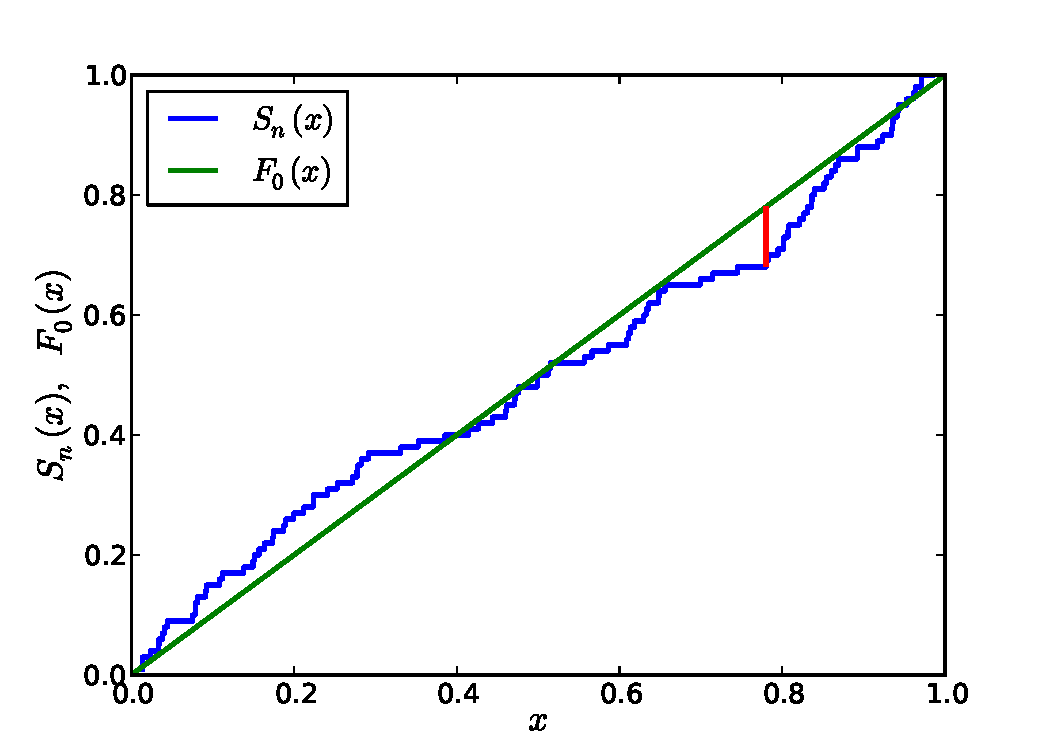
\includegraphics[width=0.75\textwidth]{edf.pdf}
  \caption[CDF for $X \sim \mathcal{U}(1, 0)$ and EDF of pseudorandom numbers from a PRNG]{Empirical distribution function $S_n(x)$ (blue line) of $n = 100$ pseudorandom numbers from PRNG, supposedly drawn from a uniform distribution, and the cumulative distribution function $F_0(x)$ (green line) expected under $H_0$. The red line marks the KS test statistic $D_n$, the greatest distance between the two lines.}
  \label{fig:edf_ex}
\end{figure}



\section{The $Z$-test\label{sec:z}}

The following section is based on \emph{Advanced statistics from an elementary point of view} \shortcite{panik2005advanced}.

The $Z$-test is a test of the hypothesis that a sample is drawn from a normal population with the mean $\mu_0$. Let $(X_1, X_2, ..., X_n)$ be a set of $n$ random variables, drawn from a normal population with a known variance $\sigma^2$, but an unknown population mean $\mu$. The sample mean is denoted $\bar{X}$, and the standard deviation of the mean is related to the standard deviation of the population by $\sigma_{\bar{X}} = \sigma / \sqrt{n}$.

We wish to determine whether the population mean $\mu$ equals a hypothesized mean $\mu_0$, i.e.,
\begin{equation}
H_0: \, \mu = \mu_0.
\end{equation}
We consider here only the two-sided alternative hypothesis,
\begin{equation}
H_1: \, \mu \ne \mu_0.
\end{equation}
The test statistic used is the standard score, 
\begin{equation}\label{eq:Z}
Z = \frac{\bar{X} - \mu_0}{\sigma_{\bar{X}}}
\end{equation}
which, under $H_0$, has a standard normal distribution $\mathcal{N}(0,1)\label{eq:normal}$. The $p$-value of the two-sided $Z$-test is the probability of finding a value of $Z$ as extreme or more extreme than the observed value $z$ under $H_0$, i.e., 
\begin{eqnarray}
\text{$p$-value} &=& \Prob{Z \le -\lvert z \rvert}
                 +\Prob{Z \ge \lvert z \rvert} \\
               &=& 2\Prob{Z \ge \lvert z \rvert}.
\end{eqnarray}

If the data set consists of a single random variable X, the test statistic becomes 
\begin{equation}\label{eq:Z}
Z = \frac{X - \mu_0}{\sigma}.
\end{equation}

The $Z$-test can only be used for data that can be approximated by a normal distribution. The central limit theorem is typically invoked to justify the approximation. 



\clearchapter





